\documentclass[aspectratio=1610]{beamer}
\usepackage{graphicx,amsmath,amsthm,verbatim,bm}
\usepackage{longtable}
%\usetheme{Copenhagen}
%\useoutertheme[{options}]{tree}
%\setbeamertemplate{footline}[page number]
%\useoutertheme{infolines}
%\setbeamertemplate{headlirne}{}
\useinnertheme{circles}
\usepackage{comment}
\setbeamertemplate{caption}[numbered]

\newcommand{\tth}   {\mbox{$\theta$}}
\newcommand{\thh}   {\mbox{$\theta$}}
\newcommand{\su}   {\mbox{$\sigma^2$}}
\newcommand{\so}   {\mbox{$\sigma_0^2$}}
\newcommand{\ko}   {\mbox{$\kappa_0$}}
\newcommand{\no}   {\mbox{$\nu_0$}}
\newcommand{\mo}   {\mbox{$\mu_0$}}
\newcommand{\ti}   {\mbox{$\tilde{x}$}}
\newcommand{\la}   {\mbox{$\lambda$}}
\newcommand{\bx}   {\mbox{$\bm{x}$}}
\newcommand{\bZ}   {\mbox{$\bm{Z}$}}
\newcommand{\bX}   {\mbox{$\bm{X}$}}
\newcommand{\bY}   {\mbox{$\bm{Y}$}}
\newcommand{\bA}   {\mbox{$\bm{A}$}}
\newcommand{\ba}   {\mbox{$\bm{a}$}}
\newcommand{\bb}   {\mbox{$\bm{b}$}}
\newcommand{\bt}   {\mbox{$\bm{t}$}}
\newcommand{\bz}   {\mbox{$\bm{z}$}}
\newcommand{\bw}   {\mbox{$\bm{w}$}}
\newcommand{\bbeta}   {\mbox{$\bm{\beta}$}}

\newcommand{\be}   {\mbox{$\bm{e}$}}
\newcommand{\bu}   {\mbox{$\bm{u}$}}
\newcommand{\bv}   {\mbox{$\bm{v}$}}
\newcommand{\sig}   {\mbox{$\Sigma$}}
\newcommand{\sigx}   {\mbox{$\Sigma_{XX}$}}
\newcommand{\sigxy}   {\mbox{$\Sigma_{XY}$}}
\newcommand{\tr}   {\mbox{$\text{tr}$}}
\newcommand{\ddet}   {\mbox{$\text{det}$}}
\newcommand\independent{\protect\mathpalette{\protect\independenT}{\perp}}
\def\independenT#1#2{\mathrel{\rlap{$#1#2$}\mkern2mu{#1#2}}}

\newcommand{\Expect}[1]{\ensuremath{\mathbf{E}\left[ #1 \right]}}
%\newcommand{\Var}[1]{\ensuremath{\mathrm{Var}\left[ #1 \right]}}
%\newcommand{\Cov}[1]{\ensuremath{\mathrm{Cov}\left[ #1 \right]}}
\newcommand{\MSE}{\ensuremath{\mathrm{MSE}}}
\newcommand{\RSS}{\ensuremath{\mathrm{RSS}}}
\newcommand{\Prob}[1]{\ensuremath{\mathrm{Pr}\left( #1 \right)}}
\newcommand{\ProbEst}[1]{\ensuremath{\widehat{\mathrm{Pr}}\left( #1 \right)}}
\DeclareMathOperator*{\argmin}{argmin} % thanks, wikipedia!
\DeclareMathOperator*{\argmax}{argmax} % thanks, wikipedia!
\DeclareMathOperator*{\sgn}{sgn} % thanks, wikipedia!

\newcommand{\lam}{\lambda}
\newcommand{\bmu}{\bm{\mu}}
%\newcommand{\bx}{\ensuremath{\mathbf{X}}}
\newcommand{\X}{\ensuremath{\mathbf{X}}}
\newcommand{\w}{\ensuremath{\mathbf{w}}}
\newcommand{\h}{\ensuremath{\mathbf{h}}}
\newcommand{\V}{\ensuremath{\mathbf{V}}}
%\newcommand{\tr}{\operatorname{tr}}

%\newcommand{\bx}{\ensuremath{\mathbf{X}}}
%\newcommand{\X}{\ensuremath{\mathbf{x}}}
%\newcommand{\w}{\ensuremath{\mathbf{w}}}
%\newcommand{\h}{\ensuremath{\mathbf{h}}}
%\newcommand{\V}{\ensuremath{\mathbf{v}}}
%\newcommand{\Cov}{\text{Cov}}
%\newcommand{\Var}{\text{Var}}

\DeclareMathOperator{\var}{Var}
\DeclareMathOperator{\cov}{Cov}
\newcommand{\Var}[1]{\ensuremath{\mathrm{Var}\left[ #1 \right]}}
\newcommand{\Cov}[1]{\ensuremath{\mathrm{Cov}\left[ #1 \right]}}


\newcommand{\indep}{\rotatebox{90}{\ensuremath{\models}}}
\newcommand{\notindep}{\not\hspace{-.05in}\indep}







\usepackage{float}
\floatstyle{boxed}
\newfloat{code}{tp}{code}
\floatname{code}{Code Example}
%\usepackage{fontspec}
%\setmainfont{Tahoma}

%\newcommand{\lam}{\lambda}
%\newcommand{\bmu}{\bm{\mu}}
%%\newcommand{\bx}{\ensuremath{\mathbf{X}}}
%\newcommand{\X}{\ensuremath{\mathbf{x}}}
%\newcommand{\w}{\ensuremath{\mathbf{w}}}
%\newcommand{\h}{\ensuremath{\mathbf{h}}}
%\newcommand{\V}{\ensuremath{\mathbf{v}}}
%\newcommand{\cov}{\text{Cov}}
%\newcommand{\var{\text{Var}}}

%\DeclareMathOperator{\var}{Var}
%\DeclareMathOperator{\cov}{Cov}

%\newcommand{\indep}{\rotatebox{90}{\ensuremath{\models}}}
%\newcommand{\notindep}{\not\hspace{-.05in}\indep}

\usepackage{graphicx} %The mode "LaTeX => PDF" allows the following formats: .jpg  .png  .pdf  .mps
\graphicspath{{./PresentationPictures/}} %Where the figures folder is located
\usepackage{listings}
\usepackage{media9}
\usepackage{movie15}
\addmediapath{./Movies/}

\newcommand{\beginbackup}{
   \newcounter{framenumbervorappendix}
   \setcounter{framenumbervorappendix}{\value{framenumber}}
}
\newcommand{\backupend}{
   \addtocounter{framenumbervorappendix}{-\value{framenumber}}
   \addtocounter{framenumber}{\value{framenumbervorappendix}} 
}


%\usepackage{algorithm2e}
\usepackage[ruled,lined]{algorithm2e}
\def\algorithmautorefname{Algorithm}
\SetKwIF{If}{ElseIf}{Else}{if}{then}{else if}{else}{endif}
%\usepackage{times}
%\usepackage[tbtags]{amsmath}
%\usepackage{amssymb}
\usepackage{amsfonts}
%\usepackage{slfortheorems}
\usepackage{epsfig}
\usepackage{graphicx}
\usepackage[small]{caption}
%\usepackage[square]{natbib}
%\newcommand{\newblock}{}
%\bibpunct{(}{)}{;}{a}{}{,}
%\bibliographystyle{ims}
%\usepackage[letterpaper]{geometry}
\usepackage{color}
\setlength{\parindent}{0pt}

\usepackage{natbib}
\bibpunct{(}{)}{;}{a}{}{,}
%\usepackage{hyperref}



%\usepackage{zref-savepos}
%
%\newcounter{restofframe}
%\newsavebox{\restofframebox}
%\newlength{\mylowermargin}
%\setlength{\mylowermargin}{2pt}
%
%\newenvironment{restofframe}{%
%    \par%\centering
%    \stepcounter{restofframe}%
%    \zsavepos{restofframe-\arabic{restofframe}-begin}%
%    \begin{lrbox}{\restofframebox}%
%}{%
%    \end{lrbox}%
%    \setkeys{Gin}{keepaspectratio}%
%    \raisebox{\dimexpr-\height+\ht\strutbox\relax}[0pt][0pt]{%
%    \resizebox*{!}{\dimexpr\zposy{restofframe-\arabic{restofframe}-begin}sp-\zposy{restofframe-\arabic{restofframe}-end}sp-\mylowermargin\relax}%
%        {\usebox{\restofframebox}}%
%    }%
%    \vskip0pt plus 1filll\relax
%    \mbox{\zsavepos{restofframe-\arabic{restofframe}-end}}%
%    \par
%}


\usepackage{tikz}
\usetikzlibrary{arrows}

%\usepackage[usenames,dvipsnames]{xcolor}
\usepackage{tkz-berge}
\usetikzlibrary{fit,shapes}

\usepackage{calc}
%%
%% The tikz package is used for doing the actual drawing.
%\usepackage{tikz}
%%
%% In order to be able to put arrowheads in the middle of directed edges, we need an extra library.
\usetikzlibrary{decorations.markings}
%%
%% The next line says how the "vertex" style of nodes should look: drawn as small circles.
\tikzstyle{vertex}=[circle, draw, inner sep=0pt, minimum size=6pt]
%%
%% Next, we make a \vertex command as a shorthand in place of \node[vertex} to get that style.
\newcommand{\vertex}{\node[vertex]}
%%
%% Finally, we declare a "counter", which is what LaTeX calls an integer variable, for use in
%% the calculations of angles for evenly spacing vertices in circular arrangements.
\newcounter{Angle}

\newtheoremstyle{example}
{\topsep} % space above
{\topsep} % space below
{} % body font
{} % indent
{\bf} % head font
{:} % punctuation between head and body
{0.5em} % space after head
{} % manually specify head
%{\thmname{#1}\thmnumber{ #2}\thmnote{:#3}} % manually specify head

\theoremstyle{example}
\newtheorem{ex}{Example}[section]

\newtheoremstyle{definition}
{\topsep} % space above
{\topsep} % space below
{} % body font
{} % indent
{\sc} % head font
{:} % punctuation between head and body
{0.5em} % space after head
{} % manually specify head
%{\thmname{#1}\thmnumber{ #2}\thmnote{:#3}} % manually specify head

\theoremstyle{definition}
\newtheorem{defn}{Definition}[section]

\theoremstyle{rem}
\newtheorem{rem}{Remark}[section]

\newtheoremstyle{theorem}
{\topsep} % space above
{\topsep} % space below
{} % body font
{} % indent
{\sc} % head font
{:} % punctuation between head and body
{0.5em} % space after head
{} % manually specify head
%{\thmname{#1}\thmnumber{ #2}\thmnote{:#3}} % manually specify head

\theoremstyle{theorm}
\newtheorem{thm}{Theorem}[section]



%%%to add in new counter for slides in beamer

%\setbeamertemplate{footline}{
%  \leavevmode%
%  \hbox{%
%  \begin{beamercolorbox}[wd=.333333\paperwidth,ht=2.25ex,dp=1ex,center]{author in head/foot}%
%    \usebeamerfont{author in head/foot}\insertshortauthor~~(\insertshortinstitute)
%  \end{beamercolorbox}%
%  \begin{beamercolorbox}[wd=.333333\paperwidth,ht=2.25ex,dp=1ex,center]{title in head/foot}%
%    \usebeamerfont{title in head/foot}\insertshorttitle
%  \end{beamercolorbox}%
%  \begin{beamercolorbox}[wd=.333333\paperwidth,ht=2.25ex,dp=1ex,right]{date in head/foot}%
%    \usebeamerfont{date in head/foot}\insertshortdate{}\hspace*{2em}
%    \insertframenumber{} \hspace*{2ex} % hier hat's sich ge�ndert
%  \end{beamercolorbox}}%
%  \vskip0pt%
%}



%%%%%

\newcommand*\oldmacro{}
\let\oldmacro\insertshortauthor
\renewcommand*\insertshortauthor{
  \leftskip=.3cm
\insertframenumber\,/\,\inserttotalframenumber\hfill\oldmacro}




\excludecomment{notbeamer}
\includecomment{beamer}



\title[Bagging and Random Forests]{Bagging and Random Forests}
\author[Rebecca C. Steorts, beka@cmu.edu]{Rebecca C. Steorts} 

\institute{\normalsize Department of Statistical Science \\ Duke University\\ \vspace*{1em} Predictive Modeling}
\date{November 2015}

\begin{document}


\begin{frame}
\titlepage
\end{frame}




\frame{

While bagging can improve predictions for many regression methods, it is very useful for regression trees. To apply bagging to regression trees we:

\begin{enumerate}
\item Construct $B$ regression trees using $B$ bootstrapped training sets.
\item We then average the predictions.
\item These trees are grown deep and are not pruned. 
\item Each tree has a high variance with low bias. Averaging the $B$ trees brings down the variance. 
\item Bagging has been shown to give impressive improvements  by combining hundreds or thousands of trees in a single procedures. 
\end{enumerate}

}

\frame{
\begin{itemize}
\item We have just described bagging in a regression context to predict a quantitative outcome $Y.$ 
\item What if our outcome is qualitative? 
\item For a given test observation, we can record the class predicted by each of the $B$ trees.
\item Now take a majority vote: the overall prediction is the most commonly occurring class among the $B$ predictions. 
\end{itemize}
}


\frame{
\center
\emph{
Straightforward way to estimate the test error of a bagged model, without the need to perform CV or the validation test set approach.}

}

\subsection{Out-of-Bag Error Estimation}

\frame{
\begin{itemize}
\item Key to bagging is that the trees are repeatedly fit to bootstrapped subsets of observations. 
\item Can show that on average, each bagged tree make use of around two-third of the observations.
\begin{itemize}
\item The remaining one-third of the observations not used to fit a given bagged tree are called \emph{out-of-bag} (OOB) observations. 
\item We can predict the response for the $i$th observation using each of the trees in which that observation was OOB. 
\item This will yield approximately $B/3$ predictions for the $i$th observation. 
\end{itemize}
\item To obtain a single prediction for the $i$th observation, we can average these predicted responses (if regression is the goal). 
\item This yields a single OOB prediction for the $i$th observation. 
\end{itemize}
}
\frame{
\begin{itemize}
\item An OOB prediction can be found in this way for each of the $n$ observations, from which the overall OOB MSE (for a regression problem) or a classification error (for a classification problem) can be computed. 
\item Check the details on your own! 

\end{itemize}


}

\frame{

\begin{itemize}
\item Bagging typically results in improved accuracy over prediction using a single tree. 
\item However, the resulting model can be difficult to interpret. 
\item One advantage of decision trees is ease of interpretation. 
\item When we bag a large number of trees, we can no longer represent the resulting statistical learning procedure using a single tree 
\item It is not clear which variables are the most important. 
\item \textcolor{blue}{Bagging improves prediction accuracy at the cost of interpretability. }
\end{itemize}

}

\frame{
\begin{itemize}

\item Collection of bagged trees is much more difficult to interpret that a single tree.
\item But we can obtain a summary of the importance of each predictor us the RSS (for bagging regression trees) or the Gini index (for bagging classification trees). 
\item In the case of regression trees, we can record the total amount that the RSS decreases due to splits over a given predictor, averaged over all $B$ trees. 
\begin{itemize}
\item A large value indicates an important predictor. 
\item For classification trees, we can add up the total amount that the Gini index decreases by splits over a given predictor averaged over all $B$ trees.
\end{itemize}
\end{itemize}
}

\section{Random Forests}

\frame{
\center
\emph{Random forests provide an improvement over bagged trees by way of a small tweak that decorrelates the trees. As in bagging, we build a number of decision trees on bootstrapped training samples. }

}

\frame{

\begin{itemize}
\item When building these decision trees, each time a split is considered, a random sample of $m$ predictors is chosen as split candidates from the full set of $p$ predictors. 
\item The split is allowed to use \emph{only one} of those $m$ predictors. 
\item A fresh sample of $m$ predictors is taken at each split, and typically we take $m \approx \sqrt(p)$.
\item That is, the number of predictors considered at each split is approximately equal to, the square root of the total number of predictors.
\end{itemize}
}

\frame{
\begin{itemize}
\item Build a random forest
\begin{itemize}
\item At each split:
\item The algorithm is not allowed to consider a majority of the available predictors. 
\item What is the reasoning? 
\item Suppose one very strong predictor along with many moderately strong predictors. 
\end{itemize}

\item In the collection of bagged trees, most or all of the trees will use this strong predictor in the top split. 
\item All of the bagged trees will look very similar. \item Predictions from the bagged trees highly correlated. 
\item Averaging highly correlated trees doesn't lead to as large of a reduction in variance as averaging many uncorrelated trees. 
\item This means that bagging will NOT lead to a substantial reduction in variance over a single tree for this example. 
\end{itemize}

}

\frame{
\begin{itemize}
\item How do random forests overcome this problem? 
\item Force each split to consider only a subset of the predictors. 
\item On average, $(p-m)/p$ of the splits won't even consider a strong predictor 
\item Means other predictors have more of a chance! 
\item This process de-correlates the trees.
\end{itemize}
}

\frame{
\begin{itemize}
\item What is the main difference between bagging and random forests? 
\item It's the choice of the predictor subset size $m.$ 
\item For example, if the random forest is built using $m = p,$ then this is the same as bagging. 
\item Using a small value of $m$ in building a random forest will typically be helpful when we have a large number of correlated predictors.
\end{itemize} 
}

\section{Application to Bagging and RF's}

\frame{
\begin{itemize}
\item We perform bagging on the Boston dataset using the randomForest package in \texttt{R}. 
\item The results from this example will depend on the version of \texttt{R} installed on your computer.\footnote{Recall that bagging is a special case of a random forest with $m = p.$} 
\item We can use the randomforest() function to perform both random forests and bagging. 
\item Note that \texttt{medv} is the median value of owner-occupied homes in \$1000s.
\item The covariates can be found at \url{http://cran.r-project.org/web/packages/MASS/MASS.pdf}
\end{itemize}
}

\begin{frame}[fragile]
\scriptsize
\begin{verbatim}
library(ISLR)
library(MASS)
library(randomForest)
attach(Boston)
set.seed(1)
train <- sample(1:nrow(Boston), nrow(Boston)/2)
bag.boston <- randomForest(medv~., data=Boston, 
     subset=train,  mtry=13, importance= TRUE)
\end{verbatim}
The argument mtry=13 indicates that all 13 predictors should be considered for each split of the tree. Basically, bagging 
should be done. How well does the bagged model perform on the test set?
\end{frame}

\begin{frame}[fragile]
\scriptsize
\begin{verbatim}
> bag.boston

Call:
 randomForest(formula = medv ~ ., data = Boston, mtry = 13, 
 importantance = TRUE,      subset = train) 
               Type of random forest: regression
                     Number of trees: 500
No. of variables tried at each split: 13

          Mean of squared residuals: 11.13692
                    % Var explained: 86.52
\end{verbatim}

\end{frame}

\frame{

\begin{figure}
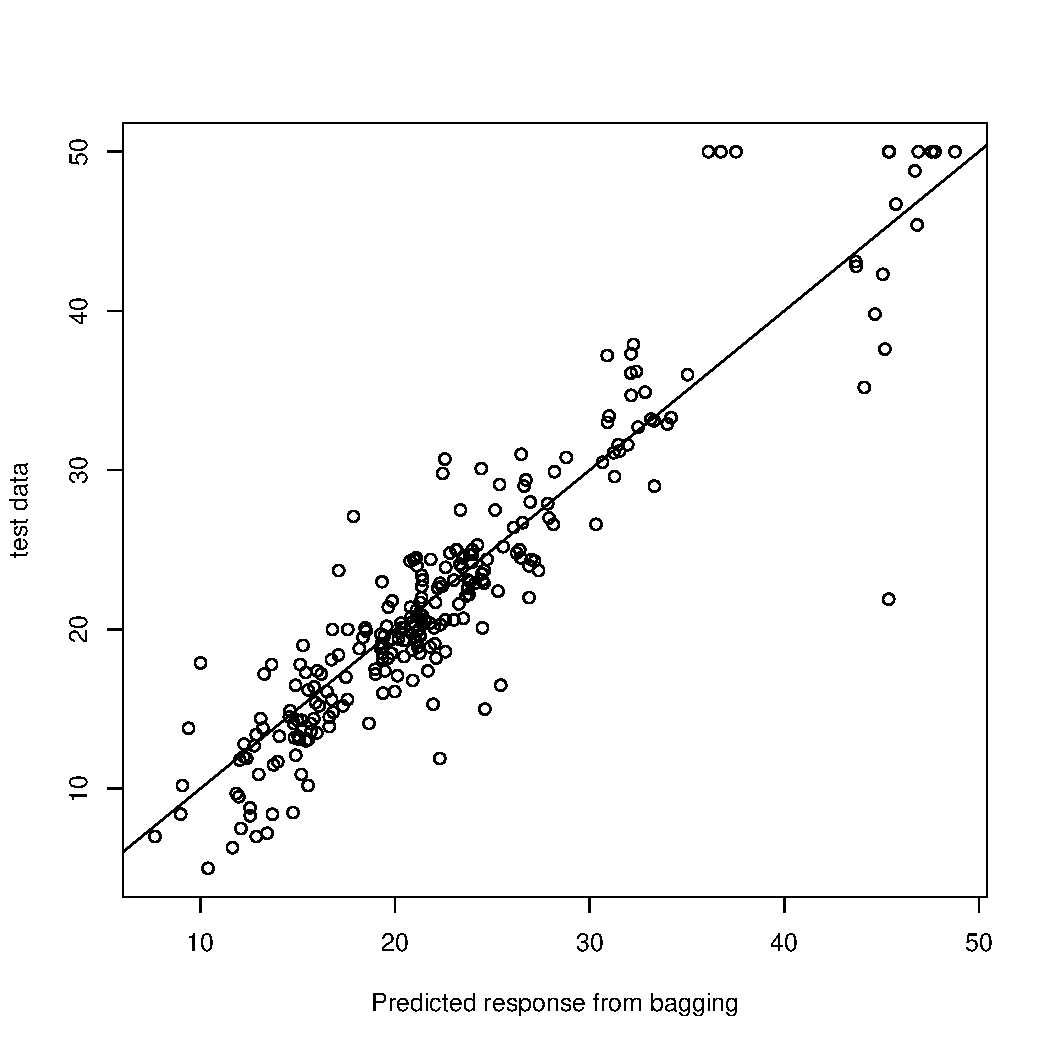
\includegraphics[scale=0.4]{bagging/boston-predict-test.pdf}
%\resizebox{\textwidth}{!}{0.6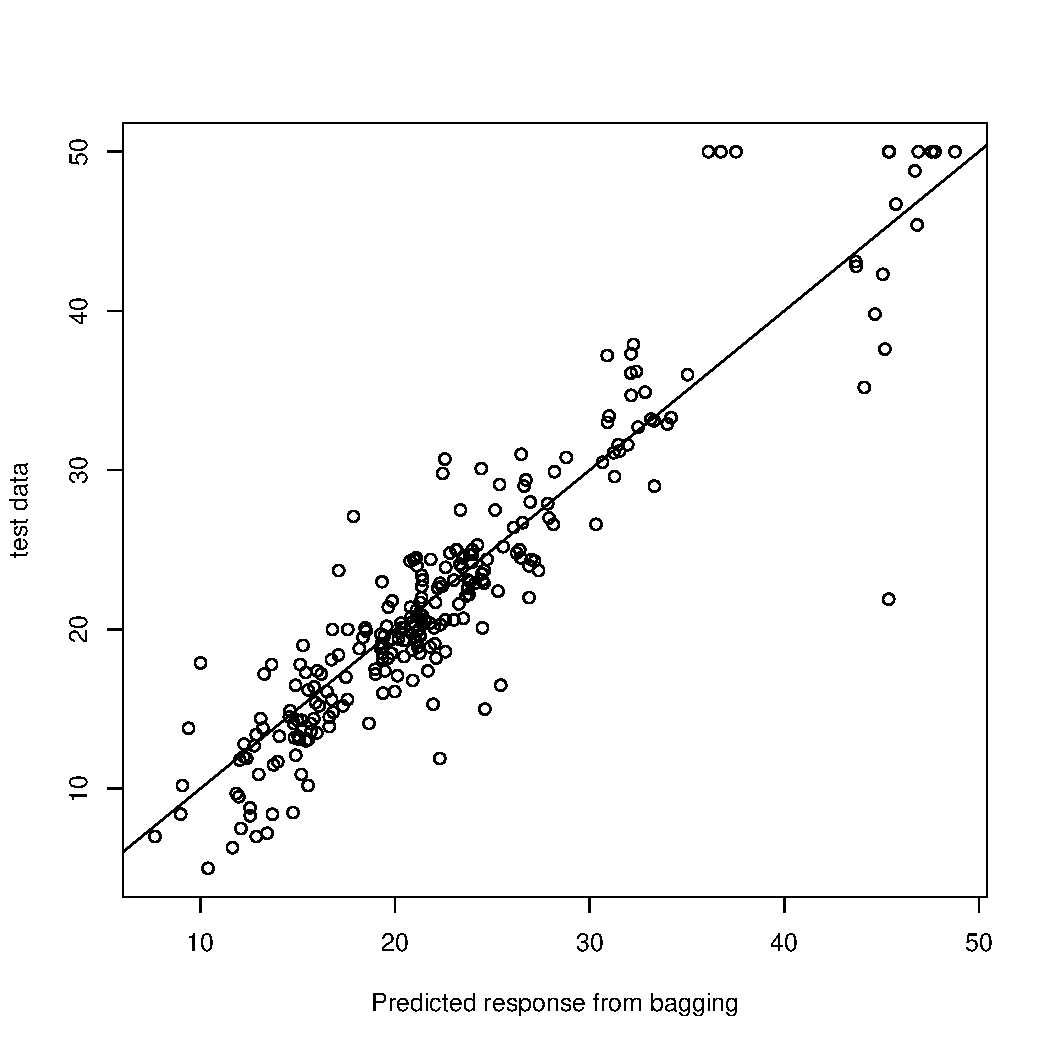
\includegraphics{bagging/boston-predict-test.pdf}}
%\begin{verbatim}
%boston.test <- Boston[-train, "medv"]
%yhat.bag <- predict(bag.boston, newdata=Boston[-train,])
%plot(yhat.bag, boston.test, xlab="Predicted response from bagging", ylab="test data")
%abline(0,1)
%mean((yhat.bag - boston.test)^2)
%\end{verbatim}
\caption{}
%\caption{Plot of the predictions of the test set of bagging versus the bagged test set. The test set MSE associated with the bagged regression tree is 12.71, about half that from using an optimally-pruned single tree. We could change the number of trees grown by randomForest() using the ntree argument. }
\label{fig:calif-lat-long-tree}
\end{figure}
}

\begin{frame}[fragile]
\textcolor{blue}{The code below shows that using tree=25 increases the test set MSE to from 11.14 to 14.28.}
\scriptsize
\begin{verbatim}
bag.boston <- randomForest(medv~., data=Boston, 
     subset=train, mtry=13, importantance = TRUE, ntree = 25)
yhat.bag <- predict(bag.boston, newdata=Boston[-train,])
mean((yhat.bag - boston.test)^2)
\end{verbatim}


\end{frame}

\frame{
\begin{itemize}
\item Growing a random forest proceeds in exactly the same way, except we use a smaller value of the mtry argument. 
\item By default, randomForest() uses $p/3$ variables when building a random forest of regression trees, and $\sqrt(p)$ variables when building a random forest of classification trees. Here we use a mtry=6. 

\item \textcolor{blue}{The test set MSE is 11.63 (compared to 14.28), indicating that random forests yield an improvement over bagging. }
\end{itemize}


}

\begin{frame}[fragile]
\scriptsize
\begin{verbatim}
set.seed(1)
rf.boston <- randomForest(medv~., data=Boston, subset=train, 
mtry=6, importantance = TRUE)
yhat.rf <- predict(rf.boston, newdata=Boston[-train,])
mean((yhat.rf - boston.test)^2)
\end{verbatim}

Using the importance() function, we can view the importance of each variable.

\begin{verbatim}
> importance(rf.boston)
        IncNodePurity
crim       1127.35130
zn           52.68114
indus      1093.92191
chas         56.01344
nox        1061.66818
rm         6298.06890
age         556.56899
dis        1371.10322
rad         111.89502
tax         442.61144
ptratio     947.18872
black       370.15308
lstat      7019.97824
\end{verbatim}

\end{frame}



\frame{
\begin{itemize}
\item Two measures of variable importance are reported. 
\item The former is based upon the mean decrease of accuracy in predictions in the out of bag samples when a given variable is excluded from the model. 
\item The latter is a measure of the total decrease in node impurity that results from splits over that variables, averaged over all trees.
\item In the case of regression trees, the the node impurity is measured by the training RSS and for classification trees by the deviance. 
\item Plots of these importance measures can be produced using the varImpPlot() function. 
\end{itemize}


}

\frame{
\frametitle{Node Purity}
\begin{itemize}
\item Splitting on those variables (rm and stat) has more of an effect on the conditional distribution of the response (y) compared to the other predictors. 
\item As the node purity increases, the conditional distribution of the response is more concentrated around particular points. 
(Recall we are doing regression and not classification).
\item In a classification setting, the node purity means that the response (y) is increasingly of the same type. 
\end{itemize}

}

\frame{
\begin{figure}
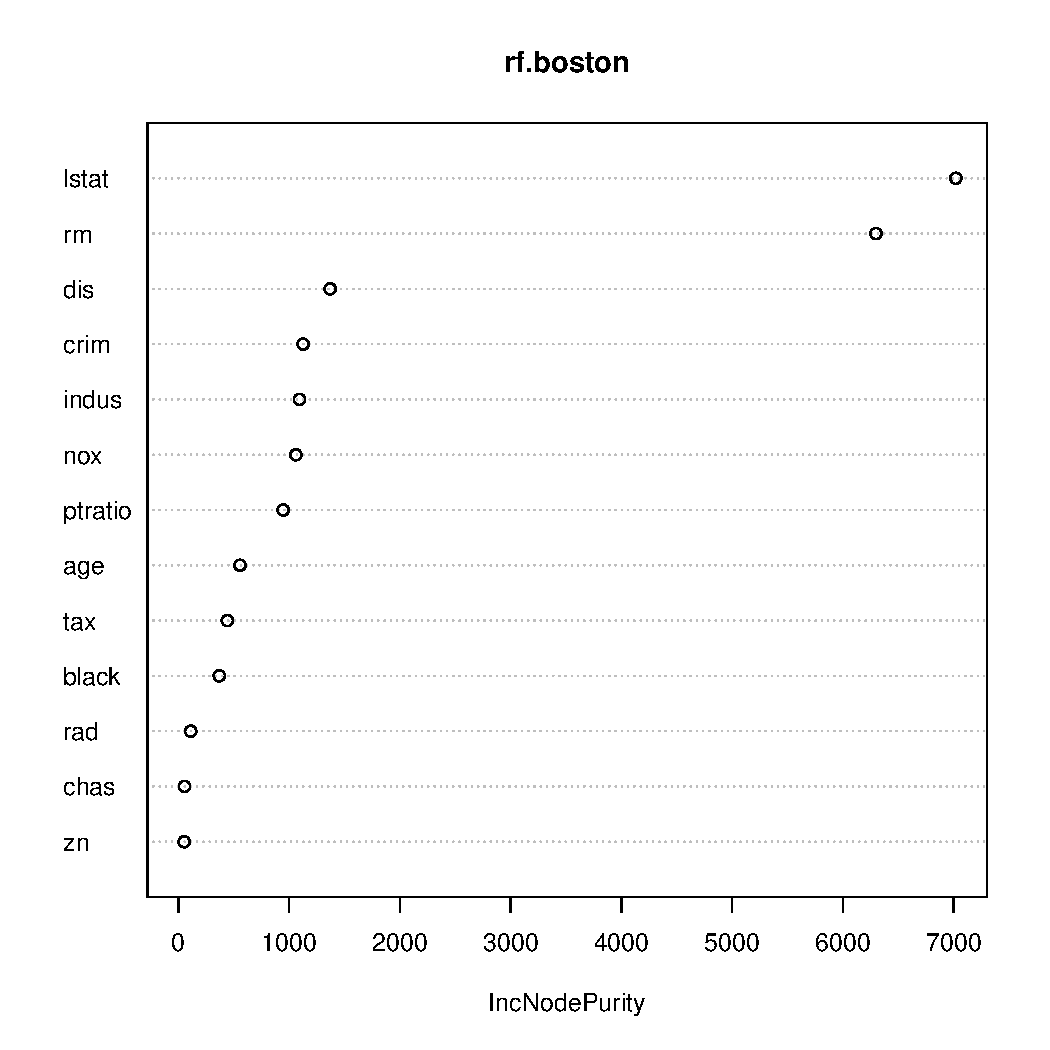
\includegraphics[scale=0.4]{bagging/varimpplot-boston.pdf}
%\resizebox{\textwidth}{!}{0.4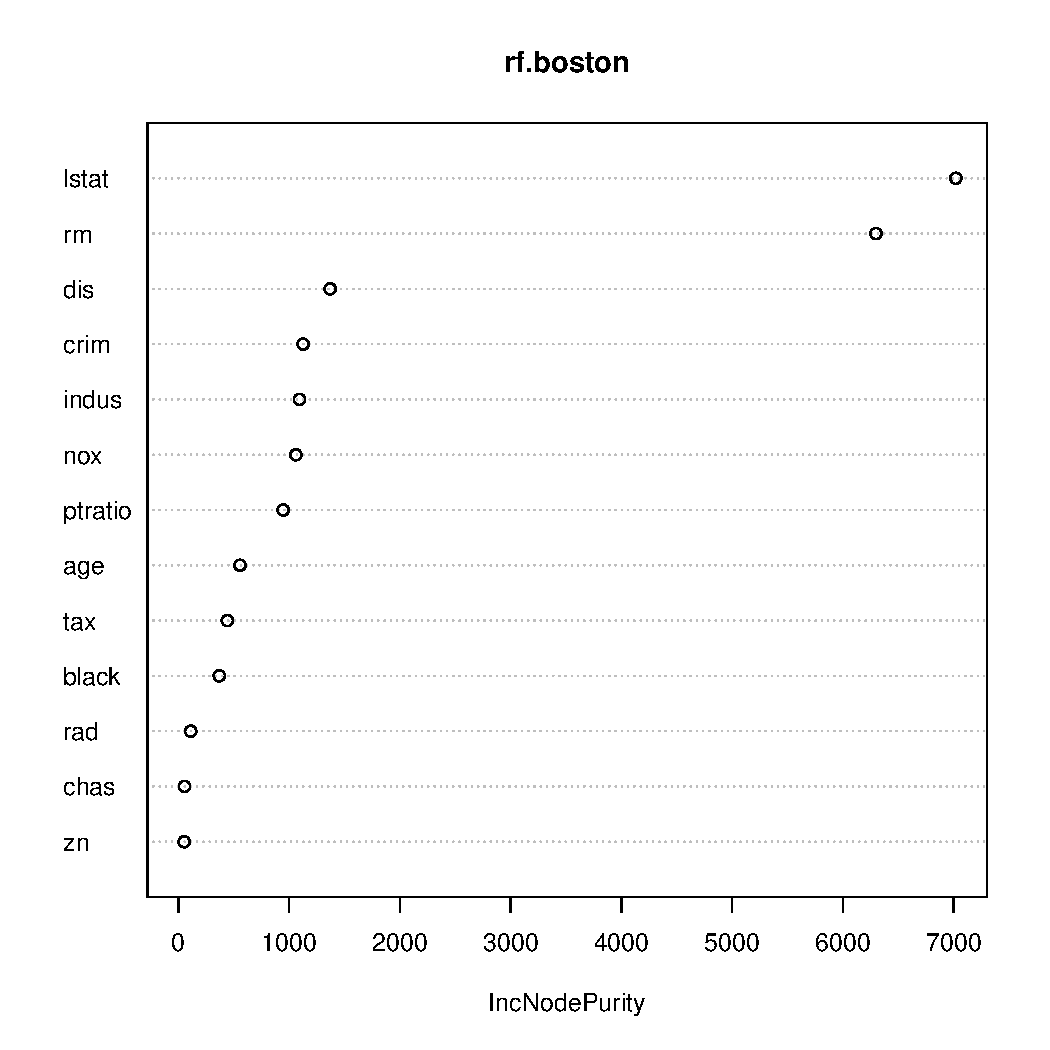
\includegraphics{bagging/varimpplot-boston.pdf}}
%\begin{verbatim}
%varImpPlot(rf.boston)
%\end{verbatim}
\caption{}
%\caption{Plot the increase in node purity and the importance of each predictor. }
\label{fig:calif-lat-long-tree}
\end{figure}

%The results indicate that across all of the trees considered in the random forest, the wealth level of the community (lstat) and the house size (rm) are by far the two most important variables.
}





\end{document}